% Figure 1: Peafowl pipeline schematic (schematic)
\begin{figure}[htbp]
\centering

\includegraphics[width=0.95\textwidth]{figures/fig1_pipeline.pdf}
\caption{Overview of the Peafowl pipeline. Input DNA sequences are decomposed into $k$-mers by Jellyfish for odd $k \in \{9, 11, \ldots, 31\}$; a binary matrix $X$ encodes the presence ($1$) or absence ($0$) of each $k$-mer in each species; the $k$-mer length maximizing the cumulative entropy over $p = 5000$ randomly sampled rows is selected as $k_\mathrm{entropy}$; and the corresponding matrix is passed to RAxML under the BINGAMMA two-state substitution model to estimate the maximum-likelihood tree topology.}
\label{fig:pipeline}
\end{figure}

% Figure 2: nRF across seven benchmark datasets (data-grounded)
\begin{figure}[htbp]
\centering
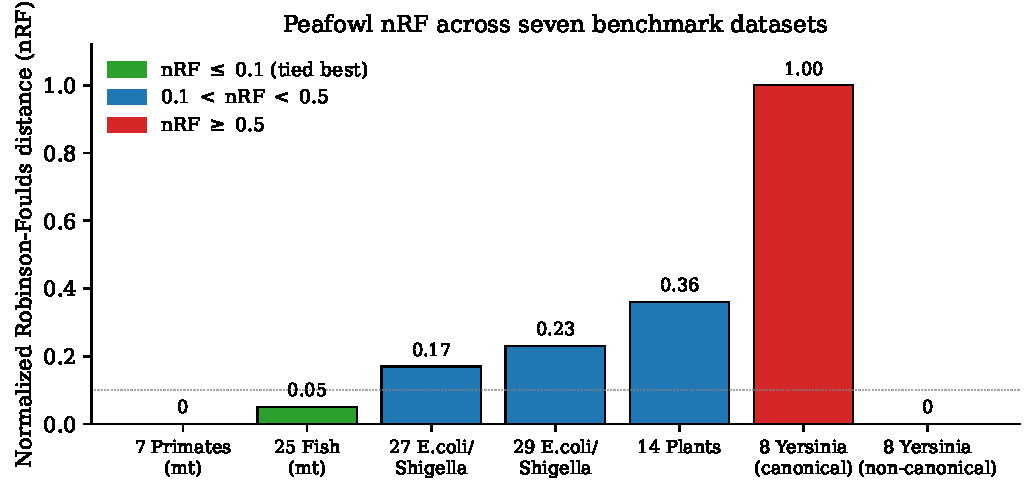
\includegraphics[width=0.95\textwidth]{figures/fig2_nrf_bar.pdf}
\caption{Normalized Robinson--Foulds (nRF) distance achieved by Peafowl on seven real benchmark datasets. Values are taken from the experimental log: $0$ on 7 Primates; $0.05$ on 25 Labroidei fish; $0.17$ on 27 E.coli/Shigella; $0.23$ on 29 E.coli/Shigella (assembled); $0.36$ on 14 plants; $1$ on 8 Yersinia under canonical $k$-mer counting; and $0$ on 8 Yersinia under non-canonical counting. Lower is better. The 14-Drosophila result (tied-best along with Skmer and phylonium, differing from the reference by a single branch) is described in the text but not plotted because a single numeric nRF value was not available in the extracted log.}
\label{fig:nrf_bar}
\end{figure}

% Figure 3: Canonical vs non-canonical counting on Yersinia (data-grounded)
\begin{figure}[htbp]
\centering
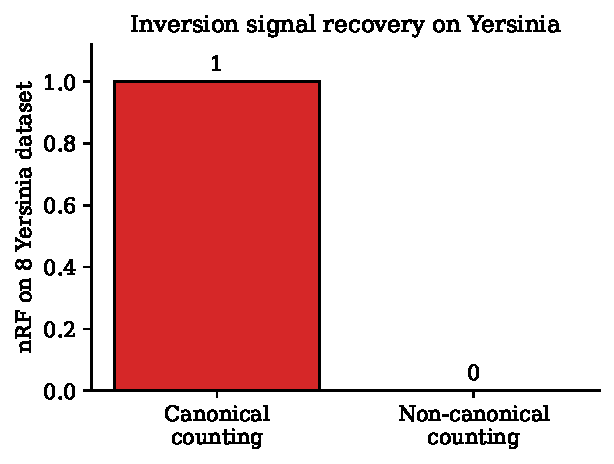
\includegraphics[width=0.55\textwidth]{figures/fig3_yersinia_canonical.pdf}
\caption{Effect of counting mode on the 8 Yersinia benchmark. Canonical $k$-mer counting, which collapses a $k$-mer and its reverse complement, yields nRF $= 1$ because the reference tree encodes genomic inversion events that are invisible once reverse complements are unified. Non-canonical counting treats a $k$-mer and its reverse complement as distinct and yields nRF $= 0$, reconstructing the reference tree exactly.}
\label{fig:yersinia}
\end{figure}
